% Options for packages loaded elsewhere
\PassOptionsToPackage{unicode}{hyperref}
\PassOptionsToPackage{hyphens}{url}
\PassOptionsToPackage{dvipsnames,svgnames,x11names}{xcolor}
%
\documentclass[
  authoryear,
  review,
  3p]{elsarticle}

\usepackage{amsmath,amssymb}
\usepackage{lmodern}
\usepackage{iftex}
\ifPDFTeX
  \usepackage[T1]{fontenc}
  \usepackage[utf8]{inputenc}
  \usepackage{textcomp} % provide euro and other symbols
\else % if luatex or xetex
  \usepackage{unicode-math}
  \defaultfontfeatures{Scale=MatchLowercase}
  \defaultfontfeatures[\rmfamily]{Ligatures=TeX,Scale=1}
\fi
% Use upquote if available, for straight quotes in verbatim environments
\IfFileExists{upquote.sty}{\usepackage{upquote}}{}
\IfFileExists{microtype.sty}{% use microtype if available
  \usepackage[]{microtype}
  \UseMicrotypeSet[protrusion]{basicmath} % disable protrusion for tt fonts
}{}
\makeatletter
\@ifundefined{KOMAClassName}{% if non-KOMA class
  \IfFileExists{parskip.sty}{%
    \usepackage{parskip}
  }{% else
    \setlength{\parindent}{0pt}
    \setlength{\parskip}{6pt plus 2pt minus 1pt}}
}{% if KOMA class
  \KOMAoptions{parskip=half}}
\makeatother
\usepackage{xcolor}
\setlength{\emergencystretch}{3em} % prevent overfull lines
\setcounter{secnumdepth}{5}
% Make \paragraph and \subparagraph free-standing
\ifx\paragraph\undefined\else
  \let\oldparagraph\paragraph
  \renewcommand{\paragraph}[1]{\oldparagraph{#1}\mbox{}}
\fi
\ifx\subparagraph\undefined\else
  \let\oldsubparagraph\subparagraph
  \renewcommand{\subparagraph}[1]{\oldsubparagraph{#1}\mbox{}}
\fi


\providecommand{\tightlist}{%
  \setlength{\itemsep}{0pt}\setlength{\parskip}{0pt}}\usepackage{longtable,booktabs,array}
\usepackage{calc} % for calculating minipage widths
% Correct order of tables after \paragraph or \subparagraph
\usepackage{etoolbox}
\makeatletter
\patchcmd\longtable{\par}{\if@noskipsec\mbox{}\fi\par}{}{}
\makeatother
% Allow footnotes in longtable head/foot
\IfFileExists{footnotehyper.sty}{\usepackage{footnotehyper}}{\usepackage{footnote}}
\makesavenoteenv{longtable}
\usepackage{graphicx}
\makeatletter
\def\maxwidth{\ifdim\Gin@nat@width>\linewidth\linewidth\else\Gin@nat@width\fi}
\def\maxheight{\ifdim\Gin@nat@height>\textheight\textheight\else\Gin@nat@height\fi}
\makeatother
% Scale images if necessary, so that they will not overflow the page
% margins by default, and it is still possible to overwrite the defaults
% using explicit options in \includegraphics[width, height, ...]{}
\setkeys{Gin}{width=\maxwidth,height=\maxheight,keepaspectratio}
% Set default figure placement to htbp
\makeatletter
\def\fps@figure{htbp}
\makeatother

\makeatletter
\makeatother
\makeatletter
\makeatother
\makeatletter
\@ifpackageloaded{caption}{}{\usepackage{caption}}
\AtBeginDocument{%
\ifdefined\contentsname
  \renewcommand*\contentsname{Table of contents}
\else
  \newcommand\contentsname{Table of contents}
\fi
\ifdefined\listfigurename
  \renewcommand*\listfigurename{List of Figures}
\else
  \newcommand\listfigurename{List of Figures}
\fi
\ifdefined\listtablename
  \renewcommand*\listtablename{List of Tables}
\else
  \newcommand\listtablename{List of Tables}
\fi
\ifdefined\figurename
  \renewcommand*\figurename{Figure}
\else
  \newcommand\figurename{Figure}
\fi
\ifdefined\tablename
  \renewcommand*\tablename{Table}
\else
  \newcommand\tablename{Table}
\fi
}
\@ifpackageloaded{float}{}{\usepackage{float}}
\floatstyle{ruled}
\@ifundefined{c@chapter}{\newfloat{codelisting}{h}{lop}}{\newfloat{codelisting}{h}{lop}[chapter]}
\floatname{codelisting}{Listing}
\newcommand*\listoflistings{\listof{codelisting}{List of Listings}}
\makeatother
\makeatletter
\@ifpackageloaded{caption}{}{\usepackage{caption}}
\@ifpackageloaded{subcaption}{}{\usepackage{subcaption}}
\makeatother
\makeatletter
\@ifpackageloaded{tcolorbox}{}{\usepackage[many]{tcolorbox}}
\makeatother
\makeatletter
\@ifundefined{shadecolor}{\definecolor{shadecolor}{rgb}{.97, .97, .97}}
\makeatother
\makeatletter
\makeatother
\journal{Habitat International}
\ifLuaTeX
  \usepackage{selnolig}  % disable illegal ligatures
\fi
\usepackage[]{natbib}
\bibliographystyle{elsarticle-harv}
\IfFileExists{bookmark.sty}{\usepackage{bookmark}}{\usepackage{hyperref}}
\IfFileExists{xurl.sty}{\usepackage{xurl}}{} % add URL line breaks if available
\urlstyle{same} % disable monospaced font for URLs
\hypersetup{
  pdftitle={`It Is Unbearable To Breath Here': Air Quality, Open Incineration, And Misinformation In Blantyre, Malawi},
  pdfauthor={Elizabeth Tilley; Hope Chilunga; Jonathan Kwangulero; Lars Schöbitz; Saloni Vijay; Heiko Heilgendorff; Marc Kalina},
  pdfkeywords={waste management, healthcare waste, trash burning, air
quality, Malawi, urbanisation},
  colorlinks=true,
  linkcolor={blue},
  filecolor={Maroon},
  citecolor={Blue},
  urlcolor={Blue},
  pdfcreator={LaTeX via pandoc}}

\setlength{\parindent}{6pt}
\begin{document}

\begin{frontmatter}
\title{`It Is Unbearable To Breath Here': Air Quality, Open
Incineration, And Misinformation In Blantyre, Malawi}
\author[1]{Elizabeth Tilley%
\corref{cor1}%
}
 \ead{tilleye@ethz.ch} 
\author[2]{Hope Chilunga%
%
}
 \ead{hchilunga@poly.ac.mw} 
\author[]{Jonathan Kwangulero%
%
}
 \ead{kwangerlo@gmail.comm} 
\author[1]{Lars Schöbitz%
%
}
 \ead{lschoebitz@ethz.ch} 
\author[1]{Saloni Vijay%
%
}
 \ead{svijay@ethz.ch} 
\author[3]{Heiko Heilgendorff%
%
}
 \ead{heiko.heilgendorff@gmail.com} 
\author[1]{Marc Kalina%
%
}
 \ead{mkalina@ethz.ch} 

\affiliation[1]{organization={ETH Zurich, Department of Mechanical and
Process Engineering},addressline={Global Health Engineering,
Clausiusstrasse
37},city={Zurich},country={Switzerland},countrysep={,},postcode={8092},postcodesep={}}
\affiliation[2]{organization={Malawi University of Business and Applied
Sciences, Department of Environmental
Health},city={Blantyre},country={Malawi},countrysep={,},postcodesep={}}
\affiliation[3]{organization={University of KwaZulu-Natal, School of
Mathematics, Statistics and Computer
Science},city={Durban},country={South
Africa},countrysep={,},postcodesep={}}

\cortext[cor1]{Corresponding author}







        
\begin{abstract}
Blantyre, Malawi's Queen Elizabeth Central Hospital (QECH), or Queen's,
as it's known locally, is the country's largest public hospital.
However, Queen's is not served by regular municipal waste collection.
What municipal collection that is done is ad-hoc, sporadic, and based on
the hospital's available financial resources. Rather, most hospital
waste (infectious and non-infectious) is gathered by grounds staff and
openly burned, in several constantly smouldering piles, sending up
clouds of smoke. Speaking directly to an identified knowledge gap on air
quality impacts linked to trash burning and the paucity of African urban
dwellers' voices on air quality issues, this study employed a
mixed-methods approach to both quantitatively measure the air quality
around QECH, and to qualitatively investigate the perceived impacts
amongst staff and caregivers. Low-cost sensors measuring particulate
matter (PM) with particle sizes less than 10 µm (PM\textsubscript{10})
and less than 2.5 µm (PM\textsubscript{2.5}), expressed as the mass of
PM per volume of air (µg PMx/m\textsuperscript{3} air) were recorded
every 5 minutes at 8 locations across the QECH for 2 months. Qualitative
data collection consisted of 56 interviews with patients, caregivers and
hospital staff (including janitorial and maintenance staff, nurses,
doctors, and administrators). Our results show that safe air quality
thresholds are consistently exceeded across space and time and that the
most problematic air quality surrounds the shelter for caregivers and
those receiving treatment for HIV/AIDs. Moreover, staff and visitors are
severely impacted by the poor air quality within the space, but feel
powerless to make changes or address complaints. Waste management
interventions are desperately needed lest the patients who arrive at
Queen's leave with more health issues than the ones with which they
arrived.
\end{abstract}



\begin{highlights}
\item Low-cost monitors were used to assess air quality at Malawi's
largest hospital\item Open waste burning is physically extensive and
temporally frequent across the hospital campus\item Air quality measured
as PM\textsubscript{2.5} and PM\textsubscript{10} consistently exceeded
even the most hazardous levels\item The most exposed locations were
where guardians of patients stay and the HIV clinic
\end{highlights}


\begin{keyword}
    waste management \sep healthcare waste \sep trash burning \sep air
quality \sep Malawi \sep 
    urbanisation
\end{keyword}
\end{frontmatter}
    \ifdefined\Shaded\renewenvironment{Shaded}{\begin{tcolorbox}[boxrule=0pt, frame hidden, borderline west={3pt}{0pt}{shadecolor}, interior hidden, enhanced, breakable, sharp corners]}{\end{tcolorbox}}\fi

\hypertarget{introduction}{%
\section{Introduction}\label{introduction}}

Built in 1964, Malawi's year of independence, Queen Elizabeth Central
Hospital (QECH), or Queen's, as it's known locally, is the country's
largest public hospital. Designed in the Tropical Modernism style of
architecture popular within Africa in the late colonial period, Queen's
open-plan form sprawls across a broad swath of central Blantyre, with
dozens of wards, specialised facilities, and administrative buildings,
linked together by a bewildering maze of covered walkways. A hive of
around-the-clock activity, Queen's bustles from dawn to dusk with a
constant stream of patients, drawn from across the country, and
maintains a city-like feel even after dark as staff and stay-in family
members cook and care for their in-patient dependants. Yet, for the
first-time visitor, it's not the architecture or the crowds that are the
most striking when entering the grounds, but the smell. Immediately
noticeable, even from the road outside the hospital, Queen's is
smothered by an acrid-smelling, white smoke, which hangs over the
grounds day and night: the product of several constantly burning fires
spread across the campus. Breathing this air, when a significant amount
of burning is occurring, primarily at night when the smoke is less
visible, can be incredibly uncomfortable. Moreover, the tropical
architecture, designed to let air and light circulate, means that even
indoors, within patient wards, surgery, and treatment areas, the air
quality can also be unbearable. Poor air quality associated with
burning, through released particulate matter (PM), has been linked to
multiple negative health outcomes like asthma, heart disease, heart
failure, stroke, and cancer among others
\citep{anderson2012clearing, bell2012assessment}. In a space of healing
and recovery, why is such burning occurring, and how can it continue to
persist?

Queen's, simply, produces an immense amount of waste that it is unable
to efficiently manage. The dozens of wards, offices, and kitchens,
serving the hundreds of patients and staff, generates considerable
infectious medical waste, mixed domestic and office waste, and kitchen
waste, which needs to be removed and disposed of daily. Some individual
wards implement waste separation, binning medical wastes separately from
general waste, however separation ends at the point of collection.
Queen's is not served by regular municipal waste collection. What
municipal collection that is done is ad-hoc, sporadic, and based on the
hospital's available financial resources. Rather, most hospital waste
(infectious and non-infectious) is gathered by grounds staff and burnt
at the hospital's incinerator, located at a central point within the
hospital campus\footnote{Sharps are handled and disposed of separately.}
\citep{kalina2020this}. However, the vast majority of the deposited
waste is not incinerated, as a new incinerator provided by the Ministry
of Health in late 2019, is only able to handle a small percentage of the
hospital's waste. Furthermore, the incinerator is frequently inoperable,
under repair, or without power\footnote{There was an older incinerator
  on the grounds which failed in 2017. Between 2017 and 2021, when the
  new incinerator was commissioned, nothing was incinerated at all.}.
Rather, the waste is openly burned, in a constantly smouldering pile to
the side of the incinerator building, sending up the aforementioned
clouds of smoke, which choke the grounds
(Figure~\ref{fig-open-burning}). Innumerable other, smaller, fires,
scattered across the QECH campus (Figure~\ref{fig-map-sensors})
contribute their part, as grounds and maintenance staff habitually burn
leaves and other garden refuse. Furthermore, caregivers\footnote{Patients
  are required to bring a caregiver for in-patient hospitals stays,
  usually a family member, who assist with feeding, bathing, and all
  other non-medical services.} who reside separately on hospital
grounds, cook for themselves throughout the day and night using biomass
(charcoal or wood), and burn their own domestic waste. As a result, air
quality at the hospital is a constant source of discussion, with
patients, staff, and caregivers struggling to cope, when just breathing
is, as the quote\footnote{ID5, 2019-11-18} used in the title of this
article, `unbearable.'

Challenges with solid waste management (SWM) are not unique to Queen's,
and remain persistent globally, particularly within African nations, and
the Global South more broadly
\citep{bundhoo2018solid, sergekubanza2022exploring, muheirwe2022paradox, srivastava2015urban}.
Explanations for these disparities have centred on the on waste
generation outstripping waste management infrastructure
\citep{muheirwe2022paradox}, and the high costs of waste management
systems, which often prove unaffordable for many low-and-middle-income
countries (LMICs) \citep{guerrero2013solid, sergekubanza2022exploring}.
Waste collection is an important step within SWM systems, and is a
common barrier within LMIC contexts \citep{bundhoo2018solid}. Waste
inequalities between high-income countries (HICs) and low-income
countries (LICs) is often most pernicious and visible at the point of
collection, with some HICs achieving 100\% collection rates, while some
African nations have rates well below 50\% \citep{shi2021unbalanced}.
Inequalities persist beyond collection, however. Even once waste is
collected, municipalities in LMICs may burn or dump it in non-sanitary
landfills due to the absence of further treatment or disposal options
\citep{cook2021globala}. According to \citet{kaza2018what}, 90\% of
waste in LIC is disposed of in unregulated dumps or openly burned, while
the quantity of waste generation in these countries is expected to
triple by 2050. As a result, open waste burning, in nations like Malawi,
can be expected to become more prevalent.

\begin{figure}

{\centering 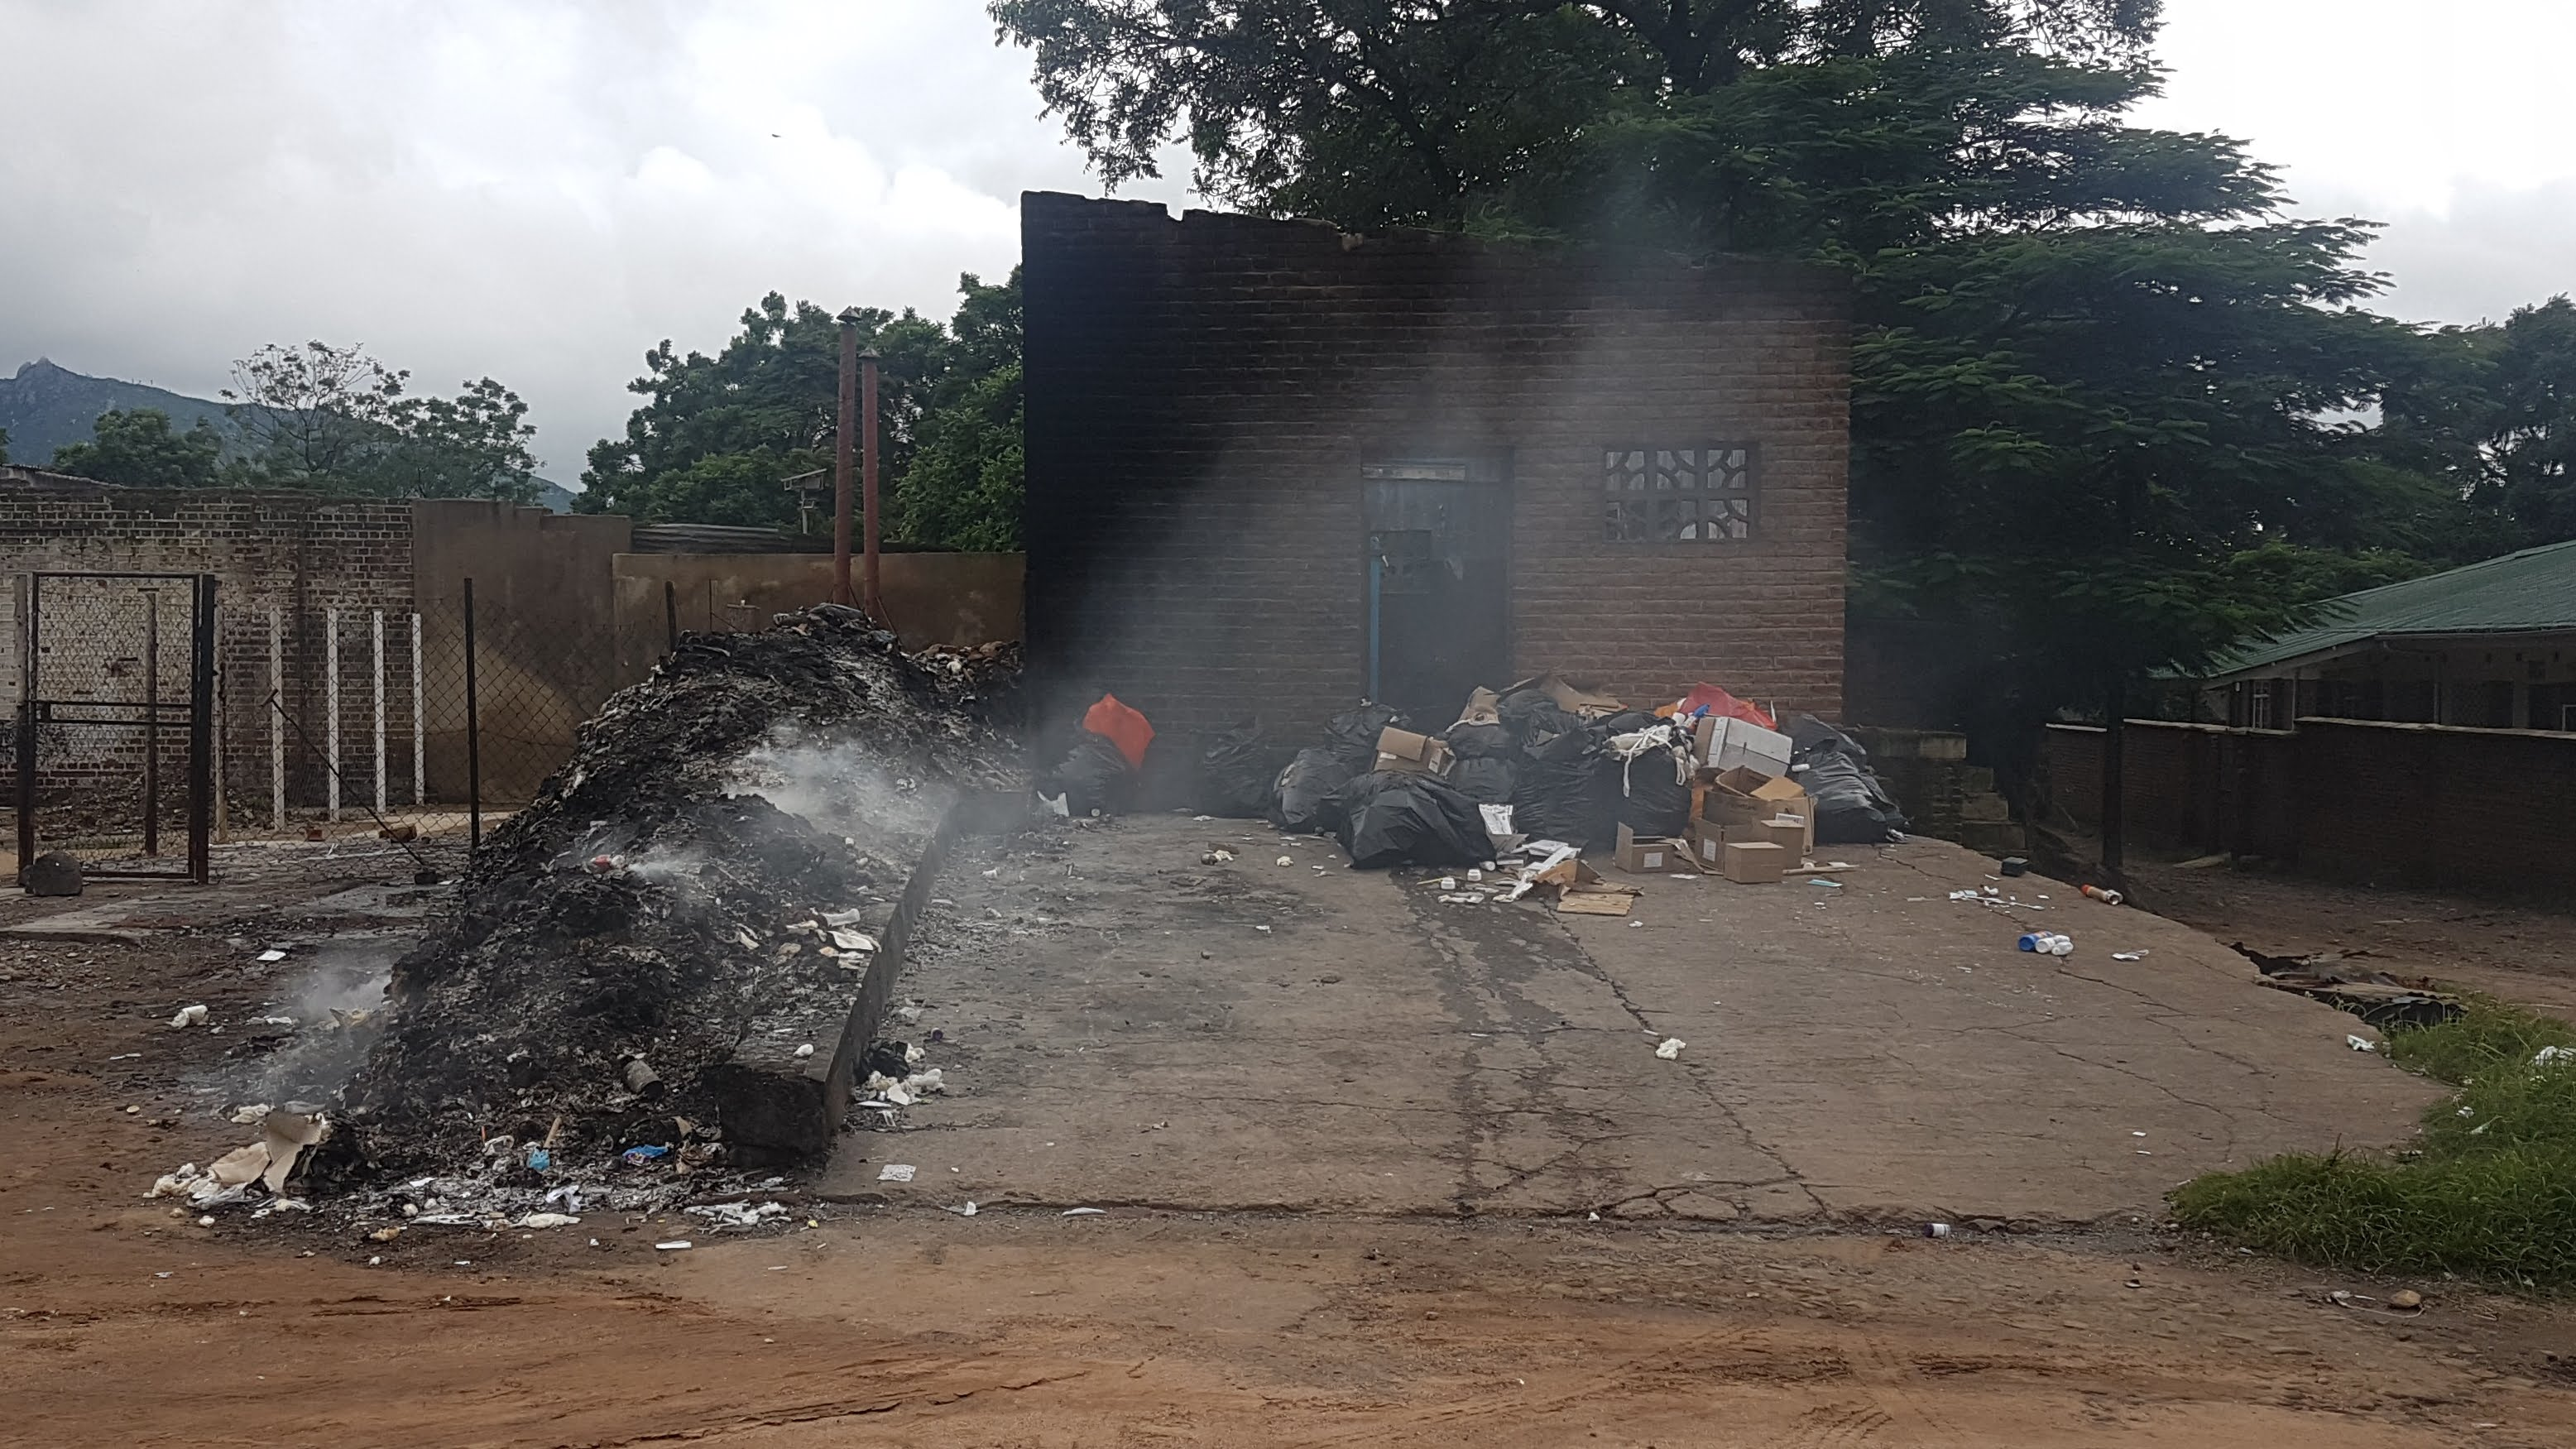
\includegraphics[width=0.8\textwidth,height=\textheight]{img/open-waste-burning-incinerator-qech.jpg}

}

\caption{\label{fig-open-burning}Open burning at QECH, with the old
incinerator building in the background (Authors).}

\end{figure}

Although hospital waste is among the common types of solid waste openly
burned in LICs (in addition to municipal solid waste, sewage sludge,
market or commercial waste, agricultural residues), the open burning of
hospital waste has not garnered as much discussion as the burning of
other waste fractions \citep{cook2021globala}. The World Health
Organisation (WHO) defines hospital, or health-care waste, as waste
generated by health-care activities, of which approximately 85\% is
general, non-hazardous waste, but the remaining 15\% can be considered
hazardous, and may be toxic, infectious, or radioactive. These
infectious fractions are commonly incinerated in both high and
middle-income countries, however in the absence of capacity, or costly
incineration or autoclave infrastructure, open burning is often a last
resort option for disposal in LIC contexts \citep{who2018healthcare}.
The open burning of biomedical waste may reduce infection risk from
potentially harmful pathogens, however, such waste may contain sharps,
radioactive waste, mercury-containing instruments, and plastics, the
open burning of which may result in the emission of dioxins, furans, and
toxic particulate matter (PM)
\citep{who2018healthcare, cook2021globala}.

Poor air quality in in African cities can be attributed to multiple
factors, including vehicular emissions, dust, or the use of low-quality
fuels for cooking, lighting, and heating, however, the open burning of
waste has been identified as one of the key contributors to air
pollution within urban areas
\citep{amegah2018proliferation, bulto2020impact}. Although open trashing
burning is a problem in LICs broadly, for instance,
\citet{wiedinmyer2014global} estimate that open trash burning
contributes to 29\% of the total global PM\textsubscript{2.5}
anthropogenic emissions, it is of particular concern in Sub-Saharan
African (SSA) cities, which are home to 19 of the world's 50 biggest
dumpsites (United Nations Development Programme, 2021). Particulate
matter, or PM, is not specific to trash burning, but rather the product
of any type of incomplete combustion and is one of the most commonly
measured indicators for air quality. PM is measured in terms of its
particle size and generally classified into PM with particle sizes less
than 10 µm (PM\textsubscript{10}) and those with sizes less than 2.5 µm
(PM\textsubscript{2.5}), while one way of measuring the severity of air
pollution is by expressing the mass of PM per volume of air (µg
PMx/m\textsuperscript{3} air). PM has been linked to multiple negative
health outcomes. Amongst particulate air pollution, PM\textsubscript{10}
and PM\textsubscript{2.5} are of particular concern as they can
penetrate deep into the lungs, and their exposure has been associated
with asthma, heart disease, heart failure, stroke, and cancer
\citep{mohapatra2014effect, xing2016impact}. As a result, the health
impacts of ambient air particle pollution may be significant, especially
for the most vulnerable. For instance, the \citet{ihme2019ambient}
estimates PM related air pollution resulted in 4.14 million deaths
worldwide (in 2019), of which, 394,000 occurred in Africa. Yet, despite
its importance, the air quality and health picture in Africa is
worryingly incomplete. For instance, the WHO only collects data from 10
African countries (covering 39 cities)
\citep{worldhealthorganization2016ambient}. Likewise, robust,
epidemiological data from and for the African context is also lacking,
though emerging data suggests strong correlations between PM and poor
health outcomes \citep{coker2018narrative, heft-neal2018robust}. Moving
forward, it is not just the air at Queen's which lacks clarity.

Utilising a mixed-methods approach, including a network of
custom-designed air quality monitors and qualitative fieldwork with
hospital staff, patients, and caregivers, the purpose of this
investigation was to gain a multi-dimensional understanding of the
impacts of the open burning of the various solid and organic waste
fractions at QECH. Specifically, this work aimed to intensively and
longitudinally measure the air quality, in particulate matter (PM), at
multiple locations at and surrounding the central burning point.
Furthermore, we also aimed to qualitatively understand how affected
individuals perceive air quality at QECH and understand potential health
impacts.

This research responds to a several specific gaps within the body of
academic air quality literature: Although there has been ample
discussion of air quality challenges in African cities
\citep{mbow-diokhane2019air, miralvarez2020scoping, petkova2013particulate, singh2021aira},
there is a paucity of data on air quality impacts linked to trash
burning. In particular, within African cities, there has been a total
dearth of scholarship on the burning of medical waste, or on air quality
within hospital contexts. Furthermore, while the voices of the citizens
of Northern cities
\citep{deguen2012new, howel2002urban, reames2019people} have been well
documented on localised air quality issues, the voices of African urban
dwellers have not been given the same consideration, and there remains a
pressing need to understand how these populations experience the impacts
of the open burning of trash within their communities and understand
potential risks.

Findings suggest that particulate matter concentrations are routinely
above the WHO guidelines and are especially worrisome at several
locations. Over the course of the two-month study, the hazardous limits
for both PM\textsubscript{10} and PM\textsubscript{2.5} were exceeded at
all locations except for the Lions Sight hospital. The limits were
exceeded fewer than 50 times at five of the locations, but the monitors
at the Lighthouse Clinic and the Guardian Shelter recorded more than 50
instances above the hazardous limits. The extremely hazardous air
quality at the Guardian shelter is mostly from cooking over open fires,
while the PM at the Lighthouse Clinic is a function of being located
directly adjacent to the smouldering waste pile.

Interviews show that patients, staff, and caregivers alike, are keenly
aware that the air quality at Queen's is poor, with most respondents
reporting frequent respiratory-related illness. Many also linked the
smoke to potential long-term health complications and expressed a belief
that the pollution could be contributing to other, more potentially
life-threatening diseases, such as asthma, cancer, and tuberculosis.
Moreover, the tropical design of hospital buildings have rendered most
coping mechanisms ineffective, with most staff only finding relief at
home: relief that is not available to the hundreds of patients and
caregivers who sleep at QECH or are unable to leave.

In many contexts, waste burning is a necessary, but sporadic event with
limited exposure. However, in the context of a large hospital, serving
the sickest and poorest, this study shows that the consistent, and
highly toxic smoke produced is an unrelenting and unnecessary burden
that must be addressed, lest the patients leave in worse condition than
in which they arrived.

\hypertarget{material-and-methods}{%
\section{Material and methods}\label{material-and-methods}}

This study utilised a mixed-methods approach to both quantitatively
measure the air quality at eight locations around QECH, and to
qualitatively investigate the perceived impacts amongst staff and
caregivers. Although the work was conducted over one sustained period in
late 2019, it must be contextualised within five years' experience of
research and activism within QECH by the authors. All relevant
permissions were obtained from QECH beforehand, through consultations
with administration and staff, and the research was approved by the
National Committee On Research in The Social Sciences And Humanities in
Malawi, Protocol NO. P.03/19/356.

\hypertarget{study-site}{%
\subsection{Study site}\label{study-site}}

The sensors were located within the QECH campus in consultation with
hospital management. The goal was to locate sensors across the campus
with a range of distances and directions from the incinerator, though
the final decision was based on accessibility, the permission of the
unit's head, and convenience. Each of the locations is briefly described
below and shown in Figure 2:

\begin{itemize}
\item
  \textbf{Lions Sight First Eye Hospital}, often shortened to
  \textbf{Lions Sight}, is the largest eye hospital in Malawi and serves
  as the main teaching eye hospital for the Kamuzu University of Health
  Sciences (formerly College of Medicine). It is staffed by 5
  consultants and a team of clinical officers and nurses. It provides a
  mix of public (no cost) and private (at cost) services.
\item
  \textbf{The Blantyre Malaria Project (BMP)}, established by Professors
  Terrie Taylor and Malcolm Molyneux, has carried out clinical research
  and patient care in the area of paediatric malaria, specifically
  cerebral malaria, for more than 30 years\footnote{BMP is credited with
    the development of the Blantyre Coma Score, which is used widely.}.
  Its research infrastructure includes an administrative team, an
  inpatient research ward, an MRI centre, and an outpatient research
  clinic in Ndirande township and in other districts outside of
  Blantyre.
\item
  \textbf{Ward 6B} is a male ward for trauma and orthopaedic patients.
  It was established as part of the original hospital design. It is a
  60-bed ward with a dedicated nursing station and treatment rooms.
\item
  \textbf{The Blantyre Lighthouse Trust Clinic}, also known as
  \textbf{Umodzi Family Centre} or simply, the \textbf{Lighthouse
  Clinic}, is one of four operating across Malawi. The clinics work in
  collaboration with the Ministry of Health (MOH) to provide integrated
  HIV testing, treatment and care for people living with HIV.
\item
  The \textbf{Moyo Nutritional Rehabilitation and Research Unit}, known
  on campus as \textbf{uMoyo}, is a 57-bed nutritional rehabilitation
  unit (NRU) for treating infants and children with severe malnutrition
  and acute illnesses. It is one of 104 operational NRUs in Malawi. It
  also has an outpatient therapeutic feeding program (OTP) for children
  with malnutrition who can be treated outside of the hospital.
\item
  \textbf{Mercy James Institute for Pediatric Surgery and Intensive Care
  (MJC)}, shortened on campus to \textbf{Mercy James}, was opened in
  2017 by the NGO Raising Malawi, which was founded by Madonna. With 3
  operating rooms and 50 beds, it is the first and only first dedicated
  paediatric surgery hospital in Malawi. Prior to its opening, QECH had
  fewer than 10 intensive care beds.
\item
  The \textbf{Administration Building} is the operational hub of the
  campus, containing mostly offices and meeting rooms.
\item
  When a patient arrives at QECH, she or he will usually arrive with a
  guardian: someone to cook for them, buy medicine, do their laundry,
  and help them bathe. The \textbf{Guardian Shelter} is a
  gender-separated concrete floor shelter for sleeping along with a
  cooking pavilion and toilet/shower block are maintained by a the local
  NGO Chira fund. Though simple, the facility is secure and offers one
  of the only free/accessible toilet facilities for visitors on the QECH
  campus.
\end{itemize}

\begin{figure}

{\centering 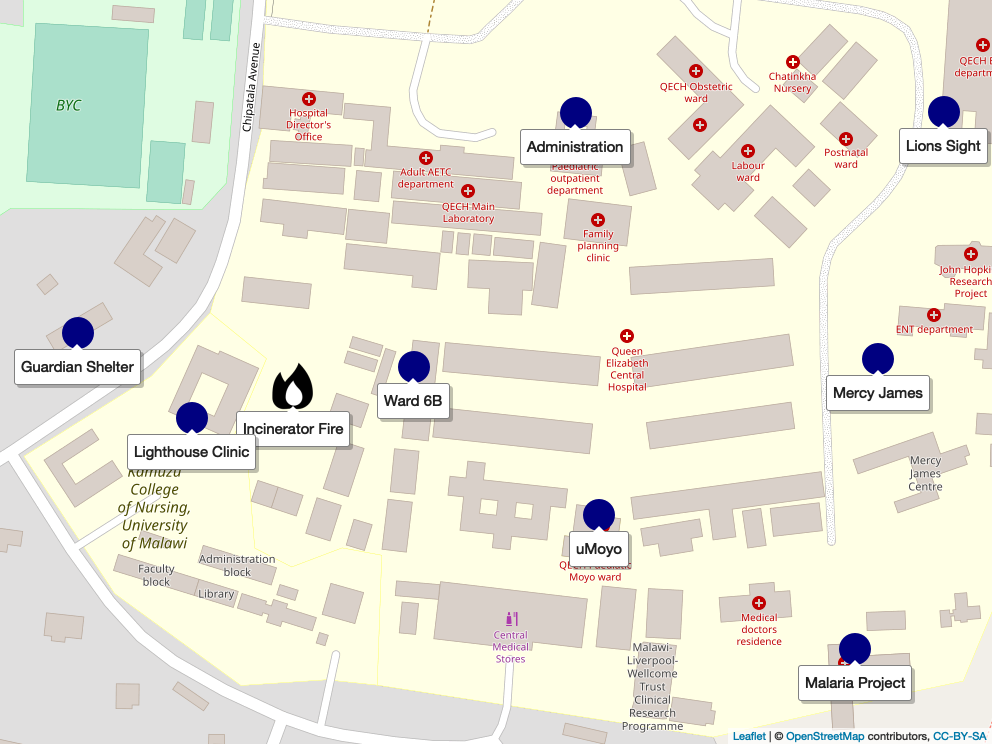
\includegraphics[width=0.8\textwidth,height=\textheight]{figs/map-sensores-qech-blantyre.png}

}

\caption{\label{fig-map-sensors}Sensor locations within QECH}

\end{figure}

\hypertarget{waste-management}{%
\subsection{Waste management}\label{waste-management}}

As the largest public hospital in the country, Queen's produces an
immense amount of waste. Hospital staff, such as doctors and nurses,
primarily generate and handle medical waste (dry, wet, sharps), which is
disposed of in separate waste bins labelled accordingly within the ward.
Hospital visitors (caretakers and patients) generate food waste and are
advised by staff to discard such waste in waste bins outside, on
hospital grounds. Cleaning staff are responsible for emptying bins and
maintaining the cleanliness of indoor and outdoor spaces. Collected bags
are temporarily stored in the sluice room, and cleaners during the night
shift are responsible for transporting the waste on wheelchairs or
trolleys to the incinerator for burning by waste disposers.

Yet, according to respondents and our own observations, waste management
procedures within the hospital are fraught with challenges which impact
the implementation of best practices. These include the lack of a
coherent hospital-wide waste management policy, insufficient waste
management training for staff, and a persistent lack of material and
financial resources. For instance, although hospital administration was
able to articulate a set of standard operating principles (SOPs) for
waste management, below the administration, doctors and nurses were
generally limited in their understanding about its contents.
Furthermore, cleaners, who are responsible for day-to-day cleansing and
waste disposal, yet rate at the bottom of the institutional hierarchy at
Queens, were unable to access or analyse hospital policy, and generally
tended to rely on, what one cleaner\footnote{ID44, 2021-01-18} described
as, ``experience'' and ``human judgement'' when handling potentially
hazardous waste. Moreover, although nearly all doctors and nurses had
prior education on waste management best practices, cleaners began their
waste handling duties without any prior waste management experience, and
although there is an orientation programme for new hires, there is no
regular refresher training or capacity building regarding waste for
existing staff, at any level.

Despite its national prominence, and international reputation for
academic medical research, Queen's is plagued by constant shortages of
human and material resources. Yet, these shortages are not shared
equally across the space, with a sharp division in cleanliness,
resources, and quality of care between public wards, supported by the
Malawi Ministry of Health, and the private wads with international
funding, such as the aforementioned Mercy James Institute. For staff,
these shortages have manifested in poor salaries, missed pay cheques,
failing infrastructure and limited supplies \citep{kalina2020this}.
Regarding waste management, these shortages have manifested in a chronic
shortage of black bags, waste containers and cleaning staff. As a
result, due to a lack of bags and storage containers, there is minimal
segregation of waste, and highly infectious items (bandages, gloves,
syringes, and other sharps) are disposed of along with non-hazardous
waste (food, newspapers, packaging). As a result, rather than
facilitating different disposal pathways for hazardous and non-hazardous
waste, all waste is mixed, necessitating more burning than would be
necessary if non-hazardous waste was diverted, and contributing to
workplace risk, with reports of accidental exposure to potentially
infected waste, including accidental pokes from improperly disposed of
sharps, common amongst hospital staff. Regardless, separation ends at
the point of collection. The hospital is not serviced by regular
municipal waste collection, and as a result, nearly all of the waste
produced by the hospital, hazardous and non-hazardous, has to be
disposed of on-site, either within the limited capacity of the hospital
incinerator, or more commonly, through open burning. As a result, the
constantly smouldering pile of waste puts forth a continuous cloud of
grey smoke, which mingling with the dozens of other fires on the
grounds, from cooking fires and burning garden waste, blankets Queen's
in a permanent cloud of foul smelling haze.

\hypertarget{measuring-air-quality}{%
\subsection{Measuring Air Quality}\label{measuring-air-quality}}

\hypertarget{hardware-and-software}{%
\subsubsection{Hardware and Software}\label{hardware-and-software}}

The PM monitoring device centres around a Raspberry Pi 3 Model B
single-board computer complete with an operating system and storage
space. The added advantage of storage space is that the data are not
lost if the internet connection breaks down. Because the Pi can only
read digital signals, we needed to include an analogue-to-digital (ADC)
converter. The amount of dust is measured by a Nova PM SDS011 High
Precision Laser sensor. This sensor measures particles at 2.5 and 10 µm
in diameter in mg/m\textsuperscript{3}. A list of the specific hardware
and software components can be found in Appendix B.

\hypertarget{installation}{%
\subsubsection{Installation}\label{installation}}

The choice of where the sensors were installed was done in collaboration
with the QECH administration, but the position of the sensors at the
individual buildings were decided by the research team. Four air quality
sensors were installed on the outside of buildings (Guardian Shelter,
Mercy James, Malaria Project, Lighthouse Clinic) while the remaining
four sensors were installed inside (Ward 6B, Administration, Lions
Sight, uMoyo). All of the sensors were mounted to a wall at a height of
approximately two metres from the ground with the help of QECH
maintenance department personnel. This height was chosen to prevent the
public from tampering with the equipment when they visit the hospital.
Additionally, we assured that each pipe that inhaled ambient air was
freely protruding in the building (room) in order to capture the air
quality.

Because connecting each unit to a power supply was not possible, each
unit was equipped with an external battery (5000 mAh) which powered the
sensor unit for three days continuously. To avoid any down time, we
changed the batteries every two days. Data were also collected from the
sensor at the time of battery replacement. The sensors were capable of
being connected to Wi-Fi, a feature which enabled wireless data access.

\hypertarget{qualitative-methods}{%
\subsubsection{Qualitative Methods}\label{qualitative-methods}}

Qualitative data collection consisted of 25 interviews with caregivers
and hospital staff (including janitorial and maintenance staff, nurses,
doctors, and administrators) conducted in October and November 2019, as
well as an additional 31 interviews conducted with staff, patients, and
caregivers in January and February 2021, spread around the hospital's
various wards and departments. Interviews were semi-structured, and
included questions on hospital waste management practices, perceived
best practices, and workplace health, safety, and risk. The first round
of interviews included specific questions on air quality, while the
second round focused on waste management more broadly. However, the
semi-structured nature of the interviews allowed for the participants to
raise topics of interest, and for unexpected themes to emerge. These
interviews are supplemented by participatory observation recorded within
detailed field notes, and supported by nearly a decade of sustained
involvement and activism by the authors in the waste management
practices of the hospital.

Interview respondents were chosen using a purposive or judgement
sampling regimen, i.e.~a subjective sampling method in which respondents
are selected based on their ability to effectively contribute to the
study's research objectives \citep{kitchin2013conducting}. All
respondents were purposively selected based on availability, willingness
to provide written, informed consent, and their individual insight into
the questions posed within the study. Interviews were conducted in the
local language (Chichewa), audio recorded, and transcribed into English.
Participation was voluntary, and responses were recorded anonymously.
Written, informed consent was obtained from each respondent prior to the
interview. The study was approved by the National Committee on Research
in the Social Sciences and Humanities (NCRSH) of Malawi; Protocol NO.
P.03/19/356. Collected data were analysed thematically and was coded
within the software programme Nvivo, which organises materials and
assists with the coding process.

\hypertarget{limitations}{%
\subsubsection{Limitations}\label{limitations}}

Though extensive and useful in understanding the conditions at QECH, the
data set would benefit from a comparison with background values. As
trash-burning is extensive throughout the city, there were no obvious
locations that could be confidently used as representative background
values. And although there were several possible areas upwind and
outside of town, the logistics and safety involved in accessing them to
change the batteries meant that the measured values at Queens could not
be compared to a stable background concentration. Knowing the wind
direction and velocity would have helped in better identifying the
potential sources of the measured PM. However, the necessary equipment
was not easily available in Blantyre at the time, and as an exploratory
study, the immediate hazards for the staff and patients at QECH are
relevant regardless of the burning source.

Knowing the exact burning locations and burning times, especially at the
incinerator and the Guardian Shelter, would have helped in better
identifying the sources and movements of the plumes. However, given the
size of the campus and it's 24-hour schedule, a much larger research
team would have been required to quantify all the burning. Finally, The
humidity, and the potential for interference was not accounted for; the
measurements were not adjusted for humidity which could affect the
values, though not enough to significantly alter the key findings and
need for immediate action.

\hypertarget{computational-reproducibility-and-data-availability}{%
\subsubsection{Computational reproducibility and data
availability}\label{computational-reproducibility-and-data-availability}}

R Statistical Software version 4.2.1, RStudio IDE version 2023.3.0.386,
and Quarto scientific publishing system version were used for
quantitative data analysis and writing of the manuscript
\citep{R-base, allaire2022quartoa, positteam2023rstudio}. A set of
additional R packages were used for data wrangling, analysis, and
visualisation
\citep{ggplot22016, lubridate2011, R-dplyr, R-forcats, R-ggplot2, R-janitor, R-leaflet, R-lubridate, R-mapview, R-readr, R-tidyr, R-waffle}.

Raw data and analysis-ready processed data is available as an R package
at \citet{R-qechairquality}. The data underlying the tables and figures
of this manuscript are contained in a repository alongside a
reproducible document that contains the analysis code and the written
narrative of the manuscript {[}TODO: manuscript software citation{]}.

\hypertarget{theorycalculation-not-applicable}{%
\section{Theory/calculation (not
applicable)}\label{theorycalculation-not-applicable}}

\hypertarget{results-and-discussion}{%
\section{Results and Discussion}\label{results-and-discussion}}

The Malawi Bureau of Standards is the national agency responsible for
setting and publishing all standards in the country. At the time of
writing, the official website (www.mbsmw.org) was not available.
However, published work that references Malawian standards
\citep{kutlarjoss2017time, mapoma2014air} indicate that the maximum 24-h
PM\textsubscript{10} value is 25 µg/m\textsuperscript{3} and the maximum
annual PM\textsubscript{2.5} value is 8 µg/m\textsuperscript{3}. There
is no daily maximum value for PM\textsubscript{2.5}. It should be noted
that both of these values are at, or below, the level-4 interim WHO
targets.

Therefore, for international comparisons and due to the lack of
comprehensive Malawian Standards, we use the WHO recommendations as a
basis of comparison for the measured values
\citep{worldhealthorganization2021who}. The relevant particulate matter
targets are presented in \textbf{?@tbl-who-targets}.

(TODO: REPLACE screenshot with actual data)

\begin{table}

\caption{\textbf{?(caption)}}\begin{minipage}[t]{\linewidth}

{\centering 

\raisebox{-\height}{

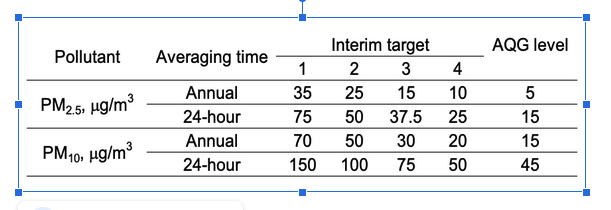
\includegraphics[width=2.04in,height=\textheight]{img/image-replace-table.png}

}

}

\end{minipage}%

\end{table}

\hypertarget{particulate-measurements}{%
\subsection{Particulate Measurements}\label{particulate-measurements}}

\hypertarget{peaks}{%
\subsubsection{Peaks}\label{peaks}}

Due to localised variation (air movement in the immediate area) and the
density of the observations, the plotted 5-minute data obscure
persistent trends. The full set of 5-minute data are plotted and
presented in Appendix A Figure~\ref{fig-five-minute-intervals}. However,
the number of measured values that exceeded the hazardous limit for both
parameters are summarised in Table~\ref{tbl-peaks}.

\hypertarget{tbl-peaks}{}
\begin{longtable}[]{@{}lrrr@{}}
\caption{\label{tbl-peaks}Peaks for both PM\textsubscript{2.5} and
PM\textsubscript{10} are the number of data points above the WHO interim
target 1 (annual) which is the least stringent; the number of
observations recorded (count) is provided for reference.}\tabularnewline
\toprule()
location & n & pm10 & pm2.5 \\
\midrule()
\endfirsthead
\toprule()
location & n & pm10 & pm2.5 \\
\midrule()
\endhead
Administration & 10900 & 171 & 0 \\
Guardian Shelter & 11032 & 4529 & 0 \\
Lighthouse Clinic & 11472 & 4365 & 0 \\
Lions Sight & 11749 & 91 & 0 \\
Malaria & 12031 & 617 & 0 \\
Mercy James & 12193 & 736 & 0 \\
Ward 6B & 11861 & 1113 & 0 \\
uMoyo & 10637 & 703 & 0 \\
\bottomrule()
\end{longtable}

Over the course of the two-month study, the hazardous limits for both
parameters were exceeded at all locations except for the Lions Sight
hospital. The limits were exceeded fewer than 50 times at five of the
locations, and only the monitors at the Lighthouse Clinic and the
Guardian Shelter recorded more than 50 instances above the hazardous
limits. At the Lighthouse Clinic, the PM\textsubscript{10} limit was
exceeded almost twice as often as the PM\textsubscript{2.5} limit, while
at the Guardian Shelter, the reverse is true. Because the Lighthouse
Clinic is within 50 m of the incinerator, the number and predominance of
PM\textsubscript{10} peaks is characteristic of incomplete combustion
and dust that is typical for the area and the open burning that occurs
there. The residents at the Guardian Shelter however are mostly cooking
within contained clay stoves that have been designed to improve
combustion of the coal and wood that is burned within them. The fewer
number of PM\textsubscript{10} peaks is a testament to this
intervention, though the frequency of PM\textsubscript{2.5} peaks is
still beyond acceptable.

\hypertarget{hour-averages}{%
\subsubsection{24-hour averages}\label{hour-averages}}

The 24-hour averaged values (logged every 5 minutes) are presented for
each location, for both PM\textsubscript{10} and PM\textsubscript{2.5}
in fig-24-hour-average. As well as dampening local variation and peaks,
the WHO air quality guidelines are also based on 24-hour averages which
are the standard against which the health risks can be judged.

Overall, PM\textsubscript{2.5} values remained below 100
µg/m\textsuperscript{3} at 6 of 8 locations (Administration, Lions
Sight, Malaria Project, uMoyo, Ward 6B, and Mercy James);
PM\textsubscript{10} values were consistently below
100µg/m\textsuperscript{3} at the same locations, but with several
average values extending slightly above, and then infrequently.

The daily averages at both the Lighthouse Clinic and the Guardian
Shelter are both consistently higher for both parameters and the two
averages closely followed the same general trends. Though the peaks at
the Lighthouse Clinic were higher than the Guardian Shelter, the low
values were consistently lower, indicating more times of little or no
burning, unlike the Guardian Shelter emissions which were relatively
constant. However, further analysis of 12 hour averages (8:00-15:59
(working hours) and 16:00-7:59 (evening)) did not indicate clear
differences between the time periods; stated differently, the data did
not clearly point to more or less burning in the day or at night.

\begin{figure}

{\centering 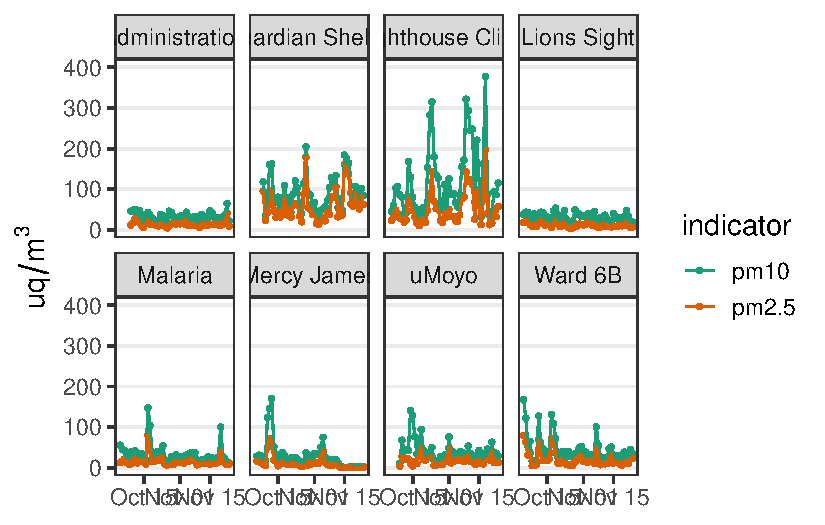
\includegraphics{manuscript_files/figure-pdf/fig-24-hour-average-1.pdf}

}

\caption{\label{fig-24-hour-average}Average 24-hour PM\textsubscript{10}
and PM\textsubscript{2.5} at 8 monitoring stations over 2 months}

\end{figure}

\hypertarget{pm-ratios}{%
\subsubsection{PM ratios}\label{pm-ratios}}

Given that the type of fuel and the type of burning (contained vs.~open)
produce very different particulate ``fingerprints'', the ratio of
PM\textsubscript{10} to PM\textsubscript{2.5} values were examined to
determine if a clear difference between locations, and therefore source,
could be identified. The results are presented in
Figure~\ref{fig-pm-ratios}.

\begin{figure}

{\centering 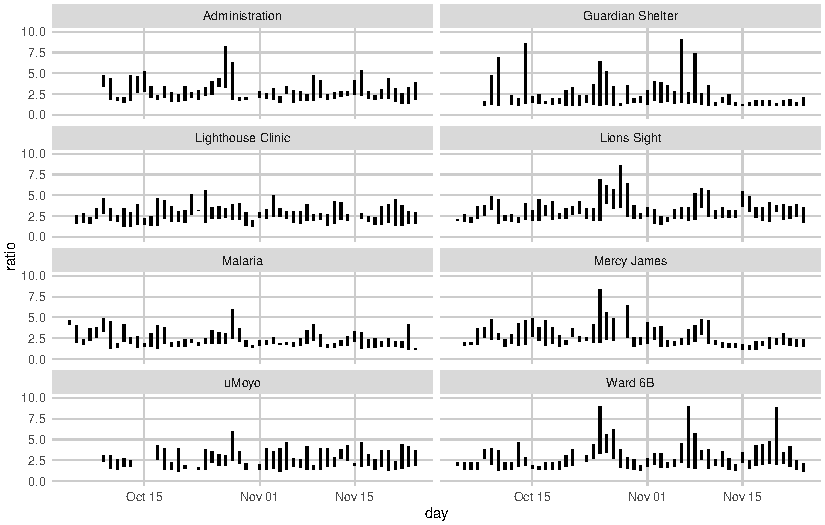
\includegraphics{manuscript_files/figure-pdf/fig-pm-ratios-1.pdf}

}

\caption{\label{fig-pm-ratios}PM\textsubscript{10}:PM\textsubscript{2.5}
values for each location. Each line shows the minimum and maximum ratio
for the day based on ratios calculated hourly. Does not include 14th to
16th October at location uMoyo due to extreme outliers.}

\end{figure}

The results presented in Figure 5 illustrate both the presence of
PM\textsubscript{10} relative to PM\textsubscript{2.5} as well as the
range of values over which that ratio is observed.

Unlike the peak values presented in Table 2, the values presented in
Figure 5 indicate the relative presence of larger (PM\textsubscript{10})
particles to smaller ones (PM\textsubscript{2.5}) regardless of their
concentration: the ratio of two low concentrations can be the same as
the ratio of two high concentrations and is therefore more indicative of
source than of proximity.

In general, the calculated ratios are concentrated between 1.25 with few
values exceeding 7.5. Three from each the Guardian Shelter and the Ward
6B exceeded 7.5 though the most values exceeding 5 were at the Guardian
Shelter. It is interesting to note that despite the large daily
variations at the Lighthouse Clinic, the parameter ratios there were
fairly consistent with few spikes, and only 2 days with ratios above 5.

An examination of the range of ratios is used to better understand the
variability within a single day. For example, several of the calculated
values at the Guardian Shelter have a range of more than 5, and one day
had a range of close to 10 i.e.~the minimum ratio recorded for that day
was close to 1 and the maximum value was over 10. The composition of
emissions recorded at that location ranged significantly, and likely
reflects a range of burning styles and/or fuel type.

\hypertarget{exposure-data}{%
\subsection{Exposure Data}\label{exposure-data}}

The relative amount of time exposed to a given category of air quality
is shown in Figure~\ref{fig-percent-exposure}. Each square represents
1\% of the measured time.

\begin{figure}

{\centering 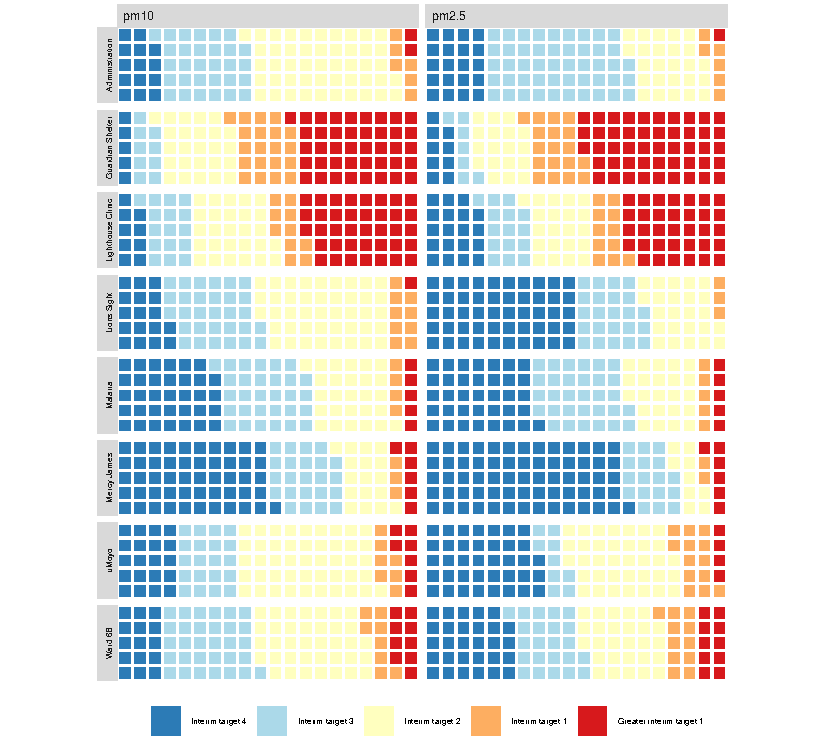
\includegraphics{manuscript_files/figure-pdf/fig-percent-exposure-1.pdf}

}

\caption{\label{fig-percent-exposure}Percentage of measured values
categorised according to WHO 2021 targets}

\end{figure}

Unsurprisingly, a majority of the air quality at the Lighthouse Clinic
and the Guardian Shelter falls at, or below, interim target 1. What is
less expected is that even though there are fewer days of hazardous or
very bad air quality at the other locations, most locations do not have
target 4 values for even half of the time. Mercy James, the Malaria
Project and Lions Sight have the largest percentages of days with air
quality meeting the interim target 4. Interim target 2 rated air
occupies an unexpectedly large proportion of the days at all locations,
indicating that although there are a few very toxic, and a few quite
good days, the majority of the air is actually neither, but still cause
for concern.

\hypertarget{the-air-we-breathe-is-not-good-perspectives-from-qech}{%
\subsection{``The Air We Breathe is Not Good'': Perspectives from
QECH}\label{the-air-we-breathe-is-not-good-perspectives-from-qech}}

As the previous section has described, the open incineration of waste at
QECH has created hazardous conditions for those occupying the space.
These risks were not lost on staff and caregivers, as interviews
demonstrated broad and near universal awareness of the poor air quality
within the hospital grounds. Overwhelmingly, within interviews, both
caregivers and staff were quick to decry the poor quality of the air,
generally without prompting. The few exceptions were those staff posted
on the peripheries of the hospital grounds, at a distance from the
spaces of incineration. However, even those who did not experience the
impacts of the burning, were aware of it, and considered themselves
fortunate to be posted in a section of the hospital where it was less of
a problem. Furthermore, according to caregivers and staff who work night
shifts, air quality can be particularly bad at night and in the early
morning, despite the smoke being less visible, due to the habit of
janitorial staff concentrating their burning during the late hours. The
poor air quality on hospital grounds is also a frequent cause for
complaint by patients and visitors, with nearly every staff member
interviewed being able to recall having received a complaint, and in
turn, complaining to administration. One of the staff\footnote{ID3,
  2019-11-18} members responsible for the burning said that he
personally, had received hundreds of complaints, but was powerless to
affect meaningful change, aside from burning at different hours, until
the incinerator could be repaired.

Nonetheless, despite this consensus that air quality caused by the
burning of waste within the hospital was a problem, significant
differences emerged between respondents over their understandings of
potential impacts, the effectiveness of various coping mechanisms, and
their problematisations linked to the burning of specific waste
materials. In addition, interviews revealed that these understandings
were informed by a significant amount of misinformation, even amongst
trained medical staff, which may contribute to them being less able to
mitigate potential risks for themselves and those who rely on their
care.

\hypertarget{impacts-problematisations-and-misinformation}{%
\subsubsection{Impacts, Problematisations, and
Misinformation}\label{impacts-problematisations-and-misinformation}}

The poor air quality within QECH was responsible, according to
respondents, for a wide array of health impacts. The most common ones
cited included: coughing and sneezing, sore throat, stinging eyes,
breathing difficulties, and persistent cold and flu. Nausea was also
mentioned, but was not a commonly described impact. Only one
respondent\footnote{ID1, 2019-11-18}, of the 26 total interviewed, did
not describe lingering health impacts which they could ascribe to the
smoke, however, they also described having chronic eye irritation, but
did not believe the smoke was a contributing factor.

In addition to these impacts, which respondents bear on a daily basis,
many also believed that the smoke could contribute to a number of more
serious, long-term health complications. For instance, nearly a quarter
of respondents raised concerns of the potential impact that the smoke
could have on patients or staff with asthma. Others flagged poor air
quality as a potential risk factor for certain cancers, lung disease, or
heart problems. For a few, the smoke posed an unknown danger, they were
not sure what types of impacts it could have, but they were sure it was
harmful in some way.

Also, understandably, given the large tuberculosis ward present within
the hospital grounds, and the high prevalence of the disease within
Malawi \citep{worldhealthorganization2019global} there was significant
concern (more than half of respondents) about the impact the poor air
quality could have on the infected. However, there also persisted a
belief among several respondents, including several nurses, that the
smoke could be a cause of the disease itself. As one staff
member\footnote{ID8, 2019-11-20} stated, ``I believe breathing this air
for a long time can cause Tuberculosis.'' This, however, was only one of
the few instances of misinformation which staff members held regarding
air quality and health. Another example, voiced by several respondents,
included a belief that some staff members were immune to ill-health
impacts of the smoke, because they had received vaccinations from the
hospital. Nonetheless, they were concerned about the impacts of the
smoke on patients and visitors, as one staff member\footnote{ID3,
  2019-11-18} expressed:

\begin{quote}
Personally, I have never experienced {[}eye discomfort{]} because I get
vaccinated and I am protected including other staff. However, we realise
that the air can badly affect other people and patients who come to this
place.
\end{quote}

Another interesting misconception that emerged, which may be tied partly
to translation and transcription, was a different cultural understanding
of smoke versus smells. More than half of the respondents appeared to
conflate the two, with some expressing a belief that it was the odour of
what was being burnt that was harmful, rather than the smoke being given
off. This has led many to specifically problematise the burning of
certain wastes, such as plastics, medicines, and other medical wastes,
which give off distinctive or less pleasant odours, as opposed to the
burning of other items, such as garden refuse, which may produce
significant smoke, and contribute to higher recorded values of
particulate matter, but produce a less pungent, or more normalised,
odour.

\hypertarget{coping-mechanisms}{%
\subsubsection{Coping Mechanisms}\label{coping-mechanisms}}

Finally, in order to manage the impacts of QECH's persistently poor air
quality, staff and visitors reported having developed a number of coping
mechanisms, designed to help them get through their daily routines.
These included staying indoors, blocking doors and windows, and taking
breaks away from hospital grounds in order to catch some breaths of
fresher air. However, for janitorial staff\footnote{ID14, 2019-11-23},
inside was not necessarily better, as several reported their indoor
workspaces as being also insufferable for long periods of time from the
smell of cleaning agents and other chemicals. Furthermore, amongst
respondents there was a general disagreement over the effectiveness of
personal protective equipment (PPE), such as face masks, towards
mitigating the impacts of the smoke. A few staff described pleading to
hospital administration for such equipment, to no avail. However, other
staff members, who do have access to PPE, noted that even face masks do
little to mitigate the impacts of the smoke, describing them as
ineffective.

Most staff, however, have been unable to find any way to mitigate the
impacts of the smoke, and only found relief once they reached home at
the end of their shift, as one of the janitorial staff described, ``we
only feel safe when we are home''. Of course, this relief is not
available for the hundreds of patients and caregivers who sleep at QECH
or are unable to leave. Ultimately, most place their hope in the
construction of the new incinerator (which had not yet been activated at
the time of the interviews), and biding their time as construction drags
on; coping as best they can. As the same member of the janitorial
staff\footnote{ID14, 2019-11-23} described, ``we are just hoping we will
start breathing good air soon, when the new incinerator is opened.''

\hypertarget{conclusions}{%
\section{Conclusions}\label{conclusions}}

The air quality, as a result of open waste burning at Queen's is poor
and not suitable for a city, let alone a hospital. Over the course of
this two-month study, the hazardous limits for both PM parameters were
exceeded at all locations except for the Lions Sight hospital. The WHO
limits were exceeded fewer than 50 times at five of the locations, and
only the monitors at the Lighthouse Clinic and the Guardian Shelter
recorded more than 50 instances above the most hazardous limit. The
composition of emissions recorded ranged significantly, analysed as the
ratio PM\textsubscript{10}:PM\textsubscript{2.5} likely reflects a range
of burning styles and/or fuel (waste) type, and no discernible trend was
observed.. Among interview respondents, there was a general consensus
that air quality caused by the burning of waste within the hospital was
a problem, although there were significant differences between
respondents over their understandings of potential impacts, the
effectiveness of various coping mechanisms, and their problematisations
linked to the burning of specific waste materials. For most, going home
or leaving the Queen's campus was the only pathway to relief, though for
patients who can not leave, endurance was the only option. This work was
originally planned as a before-and-after study: we envisioned reporting
these baseline results compared to follow-up measurements once the
long-promised incinerator was commissioned. However, nearly 4 years
later, the incinerator is rarely functional (partly for technical
reasons, partly for financial ones) and the smoke hovering over Queen's
is still thick. Waste management has long been known as an environmental
health issue, but in the case of open trash burning at a medical
facility, it becomes more: for some of the most vulnerable, especially
those with TB, asthma or other chronic disease, it could be a matter of
life or death.

\hypertarget{acknowledgements}{%
\section{Acknowledgements}\label{acknowledgements}}

The authors are grateful to the staff, patients and caregivers at QECH
for their assistance, willingness to share their views, and importantly,
perseverance in delivering the best care possible under difficult
circumstances. Moreover, we would like to acknowledge the assistance and
effort of Open Data Durban, now the Open Cities Lab, for their
assistance in constructing and programming the sensors.

\hypertarget{appendix}{%
\section*{Appendix}\label{appendix}}
\addcontentsline{toc}{section}{Appendix}

If there is more than one appendix, they should be identified as A, B,
etc. Formulae and equations in appendices should be given separate
numbering: Eq. (A.1), Eq. (A.2), etc.; in a subsequent appendix, Eq.
(B.1) and so on. Similarly for tables and figures: Table A.1; Fig. A.1,
etc.

\hypertarget{appendix-a}{%
\subsection*{Appendix A}\label{appendix-a}}
\addcontentsline{toc}{subsection}{Appendix A}

\begin{figure}

{\centering 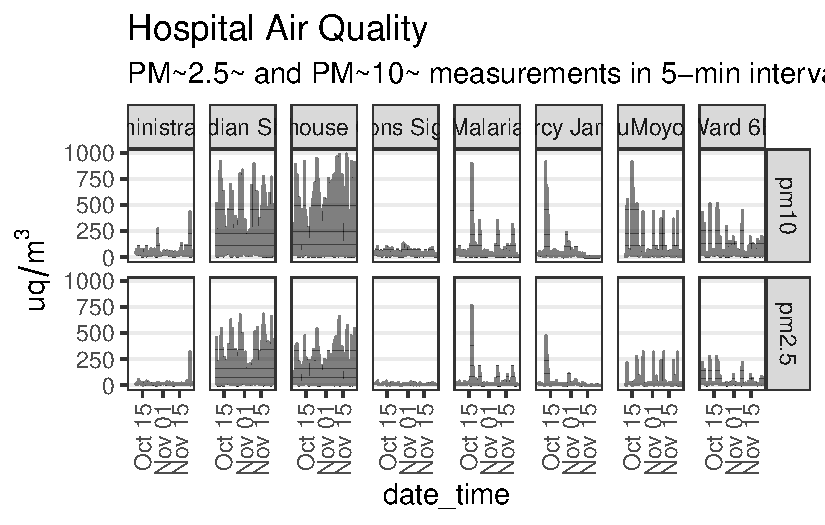
\includegraphics{manuscript_files/figure-pdf/fig-five-minute-intervals-1.pdf}

}

\caption{\label{fig-five-minute-intervals}PM\textsubscript{2.5} and
PM\textsubscript{10} values collected every 5 minutes over 10 months at
8 locations.}

\end{figure}

\hypertarget{appendix-b}{%
\subsection*{Appendix B}\label{appendix-b}}
\addcontentsline{toc}{subsection}{Appendix B}

\hypertarget{hardware-components}{%
\subsubsection*{Hardware Components}\label{hardware-components}}
\addcontentsline{toc}{subsubsection}{Hardware Components}

\begin{enumerate}
\def\labelenumi{\arabic{enumi}.}
\tightlist
\item
  Raspberry Pi 3 Model B single-board computer technical specifications:
\end{enumerate}

\begin{itemize}
\tightlist
\item
  Broadcom BCM2837 64bit Quad Core Processor powered Single Board
  Computer running at 1.2GHz 1GB RAM
\item
  BCM43438 WiFi on board
\item
  Bluetooth Low Energy (BLE) on board
\item
  40pin extended GPIO
\item
  4 x USB 2 ports 4 pole Stereo output and Composite video port
\item
  Full size HDMI CSI camera port for connecting the Raspberry Pi camera
\item
  DSI display port for connecting the Raspberry Pi touch screen display
\item
  Micro SD port for loading your operating system and storing data
\item
  Upgraded switched Micro USB power source (now supports up to 2.4 Amps)
\item
  Same form factor as the Pi 2 Model B, however the LEDs have changed
  position
\item
  RPI3-MODB-16GB-NOOBS
\end{itemize}

\begin{enumerate}
\def\labelenumi{\arabic{enumi}.}
\setcounter{enumi}{1}
\tightlist
\item
  Nova PM SDS011 Sensor
\end{enumerate}

\begin{itemize}
\tightlist
\item
  See Data Sheet attachment for technical specifications
\end{itemize}

\begin{enumerate}
\def\labelenumi{\arabic{enumi}.}
\setcounter{enumi}{2}
\tightlist
\item
  MCP3008 microchip
\end{enumerate}

\begin{itemize}
\tightlist
\item
  analogue-to-digital converter (ADC)
\end{itemize}

\begin{enumerate}
\def\labelenumi{\arabic{enumi}.}
\setcounter{enumi}{3}
\tightlist
\item
  Romoss Sense8+ 30000mAh QC Type-C
\end{enumerate}

\begin{itemize}
\tightlist
\item
  Power bank battery
\end{itemize}

\begin{enumerate}
\def\labelenumi{\arabic{enumi}.}
\setcounter{enumi}{4}
\tightlist
\item
  Pipe
\end{enumerate}

\begin{itemize}
\tightlist
\item
  clear rubber pipe attainable from any local hardware store
\end{itemize}

\begin{enumerate}
\def\labelenumi{\arabic{enumi}.}
\setcounter{enumi}{5}
\tightlist
\item
  Box
\end{enumerate}

\begin{itemize}
\tightlist
\item
  any box that can fit all the components comfortably can be used. The
  box will need to have a whole drilled in it for the pipe.
\end{itemize}

\hypertarget{software-components-and-data-management}{%
\subsubsection*{Software `components' and data
management}\label{software-components-and-data-management}}
\addcontentsline{toc}{subsubsection}{Software `components' and data
management}

\begin{enumerate}
\def\labelenumi{\arabic{enumi}.}
\tightlist
\item
  The Raspberry Pi operating system runs off of Rasbian software on a
  NOOBS scandisk.
\item
  Air quality monitoring code is written in Python using the
  \href{https://pypi.org/project/python-aqi/}{aqi library} (A library of
  algorithms to convert between AQI value and pollutant concentration).
  The code is stored on the
  \href{https://github.com/opendatadurban/hospital_stations}{Open Data
  Durban GitHub account} and is free for all to access. To be able to
  collect data, the device needs to be connected to a reliable wifi
  network, the SSID and password need to be coded onto the device during
  step 2 in the building method.
\item
  Once the whole device has been put together and placed on site, to
  access that data we use a combination of programs:
\end{enumerate}

\begin{itemize}
\tightlist
\item
  \href{https://www.putty.org/}{Putty} - this is an SSH client that we
  use to gain access to the Raspberry Pi from another computer. To be
  able to access the Raspberry Pi in question, the computer in use and
  the air quality monitoring device need to be on the same network for
  the connection to be successful.
\item
  \href{https://winscp.net/eng/download.php}{Winscp} - this is an FTP
  client that we use, in conjunction with Putty, to be able to transfer
  data files from the air quality monitoring device to one's computer.
\item
  \href{https://app.remote.it/}{Remote.it} - this is an application that
  supports remote SSH, so this is used when wanting to access data from
  a device that is not connected to the same network as the computer in
  use. Remote.it is used together with Putty and Winscp to access the
  air quality data remotely.
\end{itemize}

\hypertarget{connectionbuilding-method}{%
\subsubsection*{Connection/building
method}\label{connectionbuilding-method}}
\addcontentsline{toc}{subsubsection}{Connection/building method}

To build the sensor, we followed these steps:

\begin{enumerate}
\def\labelenumi{\arabic{enumi}.}
\tightlist
\item
  Set up the Raspberry Pi with the Rasbian software using the NOOBS
  scandisk. (insert the scandisk into the Raspberry Pi) A comprehensive
  start up guide can be found here.
\item
  Next we load the code onto the Raspberry Pi. The code can be found on
  the Open Data Durban Hospital Stations Repository Github. To use it
  you can follow the steps in the file called Initiate\_WS.txt. Once all
  the steps have been completed, the Raspberry Pi is now a device that
  can be connected to a particulate matter monitoring sensor.\\
\item
  Connect the hardware components
\end{enumerate}

\begin{itemize}
\tightlist
\item
  Connect the Raspberry Pi to the Nova PM Sensor using the break out
  board that comes with the Sensor.
\item
  Connect the battery to the Raspberry Pi via the micro port
\item
  Attach the rubber pipe to the sensor
\item
  Assemble all components inside the box, with the pipe coming out of
  the drilled hole
\item
  To prevent dirt entering the system, close off all openings between
  the pipe and the box with silicone putty
\item
  Secure box in an elevated position (not too close to the ground) and
  with the pipe facing the direction of the inflow of the air under
  investigation.
\end{itemize}


\renewcommand\refname{References}
  \bibliography{man-qechairquality.bib,packages.bib}


\end{document}
